\chapter{Các Kết Quả Thực Nghiệm}
\ifpdf
    \graphicspath{{Chapter4/Chapter4Figs/PNG/}{Chapter4/Chapter4Figs/PDF/}{Chapter4/Chapter4Figs/}}
\else
    \graphicspath{{Chapter4/Chapter4Figs/EPS/}{Chapter4/Chapter4Figs/}}
\fi
\label{chap_4}
\begin{quote}
\textit{Trong chương này, chúng tôi trình bày các kết quả thực nghiệm để đánh giá các mô hình, phương pháp và kĩ thuật được tìm hiểu mà đã trình bày ở chương trước. Bộ dữ liệu được dùng để tiến hành các thực nghiệm là bộ WMT' 13 và 14 English-German (bộ dữ liệu tiếng Anh - tiếng Đức của cuộc thi Dịch máy WMT năm 2013 và 2014). Các kết quả thực nghiệm cho thấy khi huấn luyện mô hình mà không sử dụng cơ chế Attention thì kết quả đạt được rất thấp. Các mô hình Attention Toàn cục, Attention Cục bộ, phương pháp Input feeding và kĩ thuật thay thế từ hiếm cho kết quả được cải thiện một cách vượt trội. Chúng tôi đánh giá các mô hình trên các phương diện: độ lỗi, độ đo perlexity, độ đo BLEU, đường cong học và chất lượng gióng hàng.}
\end{quote}
\section{Các thiết lập thực nghiệm}
Chúng tôi tiến hành các thực nghiệm trên bộ dữ liệu WMT' 14 English-German được cung cấp trên trang chủ của Nhóm Xử lý Ngôn ngữ Tự nhiên Đại học Stanford \cite{StanfordNMT}. Bộ dữ liệu này gồm các cặp câu được viết dưới dạng ngôn ngữ tự nhiên ở 2 ngôn ngữ là tiếng Anh và tiếng Đức. Tất cả mô hình sẽ được huấn luyện trên tập dữ liệu này. Tập dữ liệu có khoảng 4.5 triệu cặp câu (trong đó có khoảng 116 triệu từ tiếng Anh và khoảng 110 triệu từ tiếng Đức). Chúng tôi thực hiện thiết lập thực nghiệm giống với các thiết lập của bài báo của Luong, 2015 \cite{attentionThangLuong2015}.

Dữ liệu được tiến hành tiền xử lý bằng cách thực hiện tách từ đối với mỗi câu. Bộ từ vựng cho mỗi ngôn ngữ được sử dụng cho các mô hình là bộ từ vựng có 50000 từ xuất hiện nhiều nhất (có tần số lớn nhất) trong dữ liệu huấn luyện của mỗi ngôn ngữ đó. Những từ nào không nằm trong bộ từ vựng sẽ được gán cho kí hiệu $<unk>$ (từ hiếm).

Trong quá trình huấn luyện, chúng tôi lọc bỏ những cặp câu mà một trong hai câu thuộc cặp đó có chiều dài hơn 50 từ. Chúng tôi thực hiện sắp xếp tất cả câu theo chiều dài của câu giảm dần (những câu nào có chiều dài lớn nhất thì đứng đầu), sau đó lấy ngẫu nhiên các mini-batch từ những câu đã được sắp xếp. Với việc sắp xếp như vậy, tốc độ huấn luyện của mô hình được cải thiện do được tối ưu về chi phí tính toán và còn giúp mô hình học được tốt hơn.

Chúng tôi sử dụng các mô hình LSTM với mỗi LSTM có 4 tầng. Mỗi tầng LSTM có kích thước trạng thái ẩn là 1000 (đối với bộ mã hóa sử dụng bi-LSTM nên mỗi chiều của bi-LSTM sẽ có kích thước trạng thái ẩn là 500) và số chiều của word embedding là 1000. Các tham số của mô hình được khởi tạo ngẫu nhiên với phân phối đều trong đoạn $[-0,1; 0,1]$. Thuật toán để cực tiểu hóa hàm chi phí là Stochastic Gradient Descent (SGD) với kích thước của một mini-batch là 128 mẫu huấn luyện. Cách lập lịch cho hệ số học: huấn luyện 12 epochs; hệ số học ban đầu là 1.0; sau 8 epochs, hệ số học sẽ giảm đi 1 nửa sau mỗi epoch tiếp theo (epoch thứ 9 có hệ số học là 0.5, thứ 10 là 0.25, ...). Gradient của các tham số sẽ được chuẩn hóa nếu norm của chúng vượt quá 5,0. Mô hình còn sử dụng cơ chế Dropout với xác suất tắt các nơ-ron $p = 0.2$. Mỗi câu ở ngôn ngữ nguồn khi được đưa vào mô hình thì sẽ được đảo ngược trật tự. Đối với các mô hình Attention Cục bộ, kích thước cửa sổ $D = 10$.

Chúng tôi sử dụng ngôn ngữ lập trình Python và framework PyTorch dành cho Học sâu \cite{pytorchworkshop}. PyTorch hỗ trợ việc cài đặt các thuật toán Học sâu một cách thân thiện, tự nhiên giống như ngôn ngữ lâp trình Python và còn hỗ trợ xử lí tính toán song song trên GPU (Graphical Processing Units) rất mạnh mẽ. GPU mà chúng tôi sử dụng để thực hiện các thực nghiệm là NVIDIA GeForce GTX 1080 Ti. Để có thể huấn luyện một mô hình, cần đến 3-5 ngày.

Để đánh giá chất lượng dịch của các mô hình đã được huấn luyện, chúng tôi sử dụng tập dữ liệu kiểm thử \textit{newstest\_2014.en} và \textit{newstest\_2014.de} của cuộc thi WMT'14 và độ đo được sử dụng để đành giá là BLEU (BiLingual Evaluation Understudy) \cite{BLEUpaper} cùng với Perplexity. Dữ liệu validation được sử dụng là tập dữ liệu kiểm thử \textit{newstest\_2013.en} và \textit{newstest\_2013.de} của cuộc thi WMT'13.

Để đánh giá độ hiệu quả của cơ chế Attention , chúng tôi tiến huấn luyện một mô hình cơ bản (Baseline) mà không sử dụng cơ chế Attention (chỉ dùng kiến trúc Bộ mã hóa - Bộ giải mã với các LSTM). Các mô hình có sử dụng cơ chế Attention sẽ được so sánh với mô hình cơ bản này. Chi tiết của mô hình cơ bản này sẽ được trình bày trong phần tiếp theo.

\section{Kết quả thực nghiệm}
\subsection{Không sử dụng Attention và có sử dụng Attention}
Chúng tôi thực hiện đánh giá độ hiệu quả của cơ chế Attention bằng cách so sánh với mô hình không sử dụng cơ chế Attention và các mô hình có sử dụng cơ chế Attention.

Đối với mô hình không sử dụng cơ chế Attention, chúng tôi sử dụng: 
\begin{itemize}
	\item Kiến trúc Bộ mã hóa - Bộ giải mã với bộ mã hóa là bi-LSTM và bộ giải mã là uni-LSTM.
	\item Đảo ngược trật tự từ trong câu.
	\item Dropout.
\end{itemize}
Chúng tôi gọi đó là mô hình cơ bản. Đối với mô hình sử dụng cơ chế Attention, chúng tôi thiết lập mô hình như mô hình căn bản cộng với sử dụng cơ chế Attention Toàn cục với hàm tính điểm là hàm \textit{general} và có sử dụng phương pháp Input feeding, kĩ thuật thay thế từ hiếm.

Bảng \ref{tab_non-attn_vs_attn} cho thấy kết quả giữa 2 mô hình. Với cơ chế Attention, chất lượng dịch của mô hình được cải thiện rất lớn. Điểm BLEU tăng từ 15.04 đến 22.87 (+7.83). Đây là cải thiện rất lớn trong Dịch máy nơ-ron khi Dịch máy Thống kê đang dần chạm tới giới hạn. Kết quả này chứng minh được rằng cơ chế Attention rất hiệu quả trong việc giải quyết các hạn chế của kiến trúc Bộ mã hóa - Bộ giải mã với LSTM đã được trình bày ở ban đầu và cũng rất phù hợp trong việc áp dụng vào cho bài toán Dịch máy.

\begin{table}
	\centering
	\begin{tabular}{|l|l|c|} 
		\hline
		\multicolumn{1}{|c|}{ \textbf{Mô hình} }         & \textbf{Perplexity}  & \textbf{BLEU}   \\ 
		\hline
		Cơ bản                                           & 8.03                 & 15.04           \\ 
		\hline
		Cơ bản + global (general) + input feed + unk rpl & \textbf{5.22 (-2.81)}         & \textbf{22.87 (+7.83)}   \\
		\hline
	\end{tabular}
	\caption{So sánh giữa mô hình sử dụng cơ chế Attention và mô hình không sử dụng cơ chế Attention.}
	\label{tab_non-attn_vs_attn}
\end{table}

\subsection{Giữa các mô hình Attention với nhau}
Để đánh giá độ hiệu quả của các mô hình Attention với nhau, chúng tôi thực hiện huấn luyện các mô hình Attention và đánh giá chúng trên độ đo Perplexity và BLEU. Kết quả của các mô hình Attention được thể hiện trong bảng \ref{tab_attn-vs-attn}. 

% \usepackage{multirow}


\begin{table}
	\centering
	\begin{tabular}{|l|c|c|c|} 
		\hline
		\multicolumn{1}{|c|}{\multirow{2}{*}{ \textbf{Mô hình} }} & \multirow{2}{*}{\textbf{Perplexity } } & \multicolumn{2}{c|}{\textbf{BLEU } }      \\ 
		\cline{3-4}
		\multicolumn{1}{|c|}{}                                    &                                        & Trước unk rpl   & Sau unk rpl             \\ 
		\hline
		Cơ bản                                                    & 8.03                                   & 15.08           &                         \\ 
		\hline
		Cơ bản + global (dot)                                     & 6.1                                    & 18.62           & 18.81 (+0.19)           \\ 
		\hline
		Cơ bản + global (general)                                 & 4.98                                   & 19.99           & 22.33 (+2.24)           \\ 
		\hline
		Cơ bản + global (dot) + input feed                        & 5.43                                   & 19.78           & 22.24 (+2.46)           \\ 
		\hline
		Cơ bản + global (general) + input feed                    & 5.22                                   & \textbf{20.41}  & \textbf{22.87 (+2.46)}  \\ 
		\hline
		Cơ bản + local-p (general) + input feed                   & 5.43                                   & 20.37           & 22.75 (+2.38)           \\
		\hline
	\end{tabular}
	\caption{So sánh kết quả giữa các mô hình Attention với nhau.}
	\label{tab_attn-vs-attn}
\end{table}

Từ bảng kết quả cho thấy mô hình Attention Toàn cục với general product mà có sử dụng phương pháp Input feeding (global general + input feed)) có chất lượng dịch tốt nhất với điểm BLEU là 20.41 (22.87 khi dùng kĩ thuật thay thế từ hiếm). Mô hình Attention Toàn cục với hàm tính điểm \textit{dot, general} cộng với phương pháp Input feeding (global (dot) + input feed) có độ tăng điểm BLEU cao nhất khi dùng kĩ thuật thay thế từ hiếm. Kết quả này chứng minh được rằng mô hình global (general) có ý tưởng phù hợp cho cặp ngôn ngữ Anh - Đức và hoạt động hiệu quả như mong đợi trong thực tế.  Mô hình có độ đo Perplexity thấp nhất là mô hình global (general) với 4.98 perplexity. Mặc dù Perplexity hơn mô hình (global (general) + input feed) là 5.43, nhưng (global (general) + input feed) có điểm BLEU tốt nhất là 20.41, hơn 0.42 điểm. Tức là mô hình global (general) có khả năng tổng quát hóa chưa tốt.
 
Kết quả cho thấy rằng với 2 phương pháp Input feeding và thay thế từ hiếm mà chúng tôi đã trình bày ở phần trước đều góp phần tăng hiệu quả của mô hình lên rất đáng kể. Cụ thể, phương pháp Input feeding giúp mô hình global (dot) tăng điểm BLEU từ 18.62 lên 19.78 (+1.16), giúp mô hình global (general) tăng từ 19.99 lên 20.41 (+0.42). Kĩ thuật thay thế từ hiếm tăng trung bình hơn 2.0 BLEU (trừ mô hình global (dot) chỉ tăng 0.19). Các kết quả này chứng minh được rằng những ý tưởng, lý thuyết chúng tôi trình bày ở phần trước đều hoạt động tốt như mong đợi. Những phương pháp, kĩ thuật này vừa rõ ràng về mặt lý thuyết, vừa hiệu quả trong thực tế.

Về phương pháp Input feeding, có một chút hạn chế của phương pháp này về chi phí tính toán. Input feeding làm kích thước đầu vào ở các bước thời gian của uni-LSTM của bộ giải mã tăng lên theo kích thước của véc-tơ attention. Hơn nữa, về mặt cài đặt, chúng ta không tận dụng được LSTM mà đã được hỗ trợ cài đặt bởi NVIDIA. Do vậy, tốc độ huấn luyện và trong kiểm thử của mô hình khi có sử dụng cơ chế Input feeding sẽ giảm đi đáng kể, bên cạnh đó kích thước của mô hình cũng tăng lên theo.

Về kĩ thuật thay thế từ hiếm, từ kết quả cho thấy kĩ thuật này rất mạnh mẽ. Các mô hình Attention được sử dụng cùng với kĩ thuật này đều được tăng điểm BLEU hơn 2. Mô hình này chỉ có hạn chế là phải phụ thuộc vào kết quả của cơ chế Attention có tốt hay không. Kết quả cũng cho thấy rằng chất lượng mô hình Attention không tốt sẽ dẫn tới độ hiệu quả của kĩ thuật thay thế từ hiếm kém đi (mô hình global (dot)). Còn lại kĩ thuật này rất hiệu quả và tiện lợi. Thay thế từ hiếm không ảnh hưởng tới quá trình huấn luyện, do vậy mô hình không phải tốn chi phí tính toán cho kĩ thuật này trong quá trình huấn luyện và tốc độ huấn luyện không bị ảnh hưởng. 

Nhìn chung, kết quả cho thấy kĩ thuật thay thế từ hiếm cải thiện kết quả tốt hơn phương pháp Input feeding, nhưng Input feeding giúp tạo ra một mô hình Attention đủ tốt để tạo điều kiện cho kĩ thuật thay thế từ hiếm phát huy sự hiệu quả của nó.

\subsection{Phân tích đường cong học}
Phần này, chúng tôi tập trung vào so sánh các tất cả các mô hình đã thực hiện ở phương diện quá trình học bằng cách quan sát độ lỗi của mô hình bằng độ đo Perplexity trên cả tập huấn luyện và tập validation (newstest\_2013) trong quá hình huấn luyện mô hình. Điều này giúp chúng tôi biết được mô hình nào sẽ hôi tụ và tổng quát hóa tốt hơn.

\begin{figure}
	\centering
	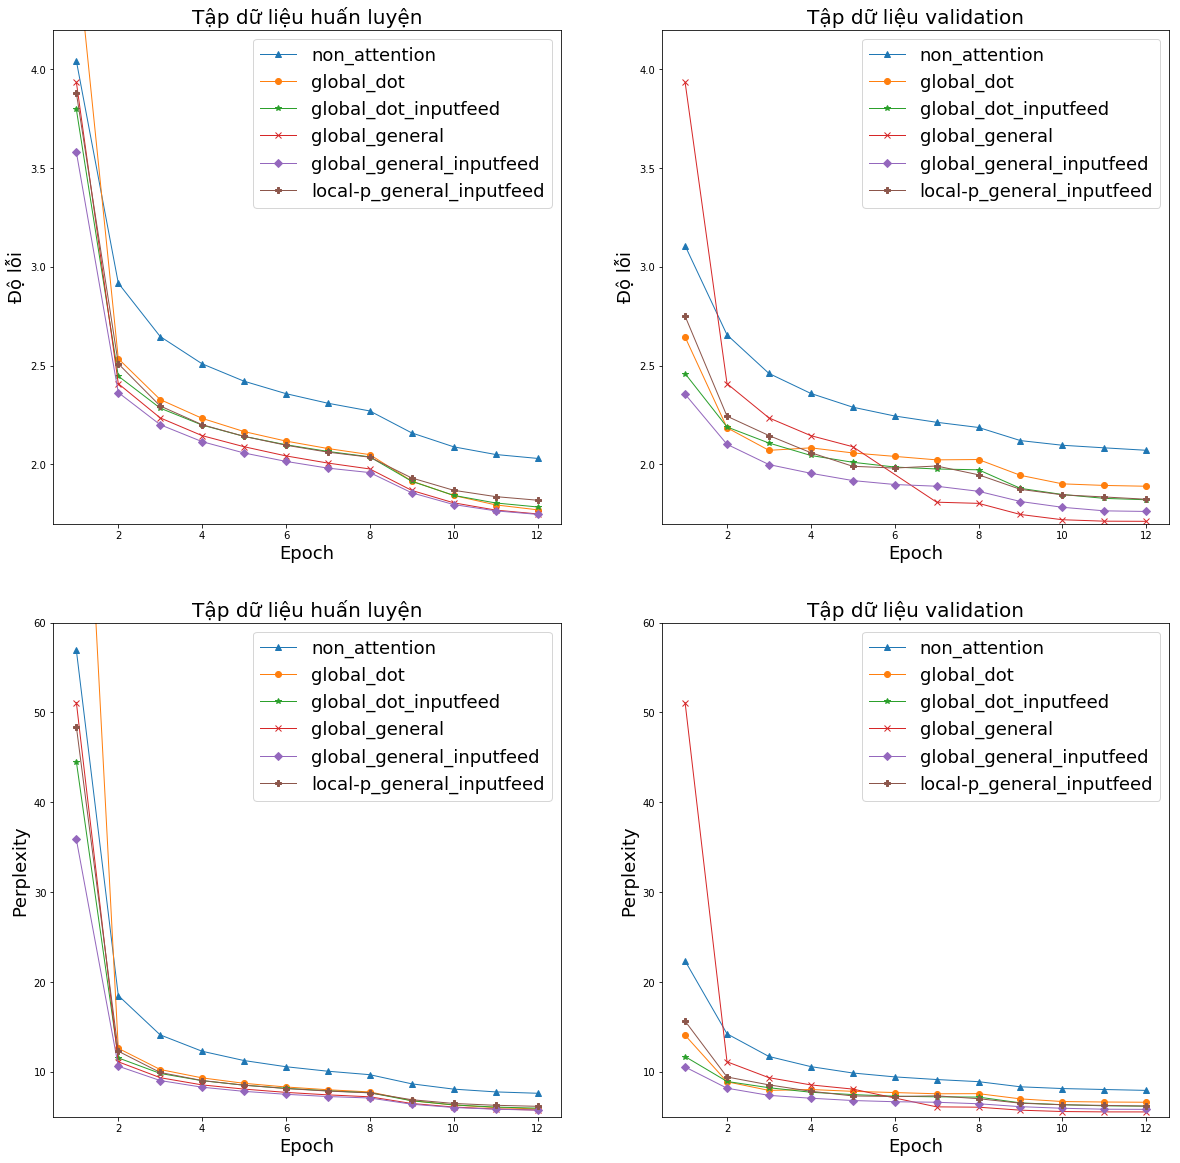
\includegraphics[width=1.0\textwidth]{train_valid_xent_ppl_scaled.png}
	\caption[Đường cong học của các mô hình]{Đường cong học của các mô hình phân tích trên độ lỗi, điểm BLEU trên tập dữ liệu huấn luyện và validation.}
	\label{fig_learning_curve}
\end{figure}

Từ đồ thị \ref{fig_learning_curve} thấy được rằng mô hình Global Attention với general product cho tốc độ hôi tụ nhanh nhất (perplexity trên tập huấn luyện giảm nhanh nhất qua các epoch), cùng với đó khả năng tổng quát hóa cũng đáng kể (perplexity trên tập validation có độ giảm tương đương). Mô hình Local Attention với general product cho khả năng tổng quát hóa tốt nhất (perplexity trên tập huấn luyện thấp hơn các mô hình khác nhưng kết quả điểm BLEU trên tập kiểm thử là tốt nhất). Trong các epoch đầu, hầu hết các mô hình có tốc độ giảm perplexity nhanh như nhau. Các mô hình Attention không sử dụng phương pháp Input feeding ở epoch đầu có perplexity cao hơn so với các mô hình sử dụng Input feeding, nhưng khi ở các epoch về sau thì tốc độ giảm perplexity giống nhau. Các mô hình Local Attention ở các epoch đầu đều có hành vi giống Global Attention, chỉ có khác nhau ở các epoch cuối cùng. Các mô hình Local Attention này ở các epoch cuối có tốc độ giảm perplexity chậm đi rõ rệt.

\subsection{So sánh với kết quả của bài báo}
Phần này chúng tôi thực hiện so sánh kết quả của chúng tôi với kết quả của bài báo \textit{Effective Approaches to Attention-based Neural Machine Translation} để đánh giá rằng mô hình của chúng tôi hoạt động có thực sự đúng không.

% \usepackage{multirow}
\begin{table}
	\centering
	\begin{tabular}{|l|c|c|c|c|} 
		\hline
		\multicolumn{1}{|c|}{\multirow{2}{*}{\textbf{Mô hình} }} & \multicolumn{2}{c|}{\textbf{Perplexity }}    & \multicolumn{2}{c|}{\textbf{BLEU }}  \\ 
		\cline{2-5}
		\multicolumn{1}{|c|}{}                                   & \textbf{KL}           & \textbf{Bài báo}     & \textbf{KL}    & \textbf{Bài báo}    \\ 
		\hline
		Cơ bản                                                   & 8.03                  & 8.1                  & 15.08          & 14.0                \\ 
		\hline
		Cơ bản + global (dot) + input feed                       & \multirow{2}{*}{5.43} & \multirow{2}{*}{6.1} & 19.78          & 18.6                \\ 
		\cline{1-1}\cline{4-5}
		Cơ bản + global (dot) + input feed + unk rpl             &                       &                      & 22.24          & 20.5                \\ 
		\hline
		Cơ bản + global (general) + input feed                   & \multirow{2}{*}{5.22} & \multirow{2}{*}{6.1} & \textbf{20.41} & 17.3                \\ 
		\cline{1-1}\cline{4-5}
		Cơ bản + global (general) + input feed + unk rpl         &                       &                      & \textbf{22.87} & 19.1                \\ 
		\hline
		Cơ bản + local-p (general) + input feed                  & \multirow{2}{*}{5.43} & \multirow{2}{*}{5.9} & 20.37          & \textbf{19.0}       \\ 
		\cline{1-1}\cline{4-5}
		Cơ bản + local-p (general) + input feed + unk rpl        &                       &                      & 22.75          & \textbf{20.9}       \\
		\hline
	\end{tabular}
	\caption{So sánh kết quả của khóa luận và bài báo.}
	\label{tab_thesis-paper}
\end{table}

Từ bảng kết quả trên cho thấy mô hình của chúng tôi hoạt động tốt. Kết quả của chúng tôi có khác với bài báo rằng hầu hết mô hình của chúng tôi đều hơn kết quả của bài báo từ 1.0 đến gần 2.0 điểm BLEU. Đặc biệt riêng với mô hình Global Attention với general product, kết quả có sự chênh lệch vô cùng lớn.

Lí do của sự khác biệt lớn này là về sự khác nhau giữa 2 ngôn ngữ và framework - Matlab và PyTorch. Matlab là một ngôn ngữ lâu đời và tại thời điểm năm 2015 mà tác giả thực hiện bài báo này thì Matlab vẫn chưa có hỗ trợ nhiều cho Học sâu và chưa tối ưu cho lập trình song song trên GPU. Do vậy, hầu hết các bước tính toán quan trọng của mô hình đều là do tác giả tự cài đặt, bao gồm cả các bước thực hiện tính đạo hàm để lan truyền ngược. Trong khi đó, PyTorch là một framework được thiết kế dành riêng cho việc hỗ trợ cài đặt các mô hình Python dựa trên ngôn ngữ Python được Facebook cùng với các trường đại học, công ty v.v... hỗ trợ phát triển. Do vậy, về mặt ý tưởng và được cài đặt khá giống nhau trên mã nguồn Matlab và Python nhưng các phần lõi của mô hình được cài đặt lại khác nhau.

\subsection{Chất lượng gióng hàng của mô hình}
Trong phần này chúng tôi trình bày về một trong những lợi ích quan trọng của các mô hình Attention là khả năng trực quan hóa những gì mô hình đã học được. Từ khi Học sâu ra đời, bên cạnh sự thành công rực rỡ trong việc giải quyết các bài toán phổ biến thì mạng Học sâu có hạn chế rất lớn về khả năng diễn dịch kết quả. Do khả năng tự học các đặc trưng, khi mạng Học sâu xuất ra các kết quả, mọi người hầu như không thể giải thích được lí do vì sao mô hình cho ra kết quả như vậy. Vì thế, mạng Học sâu không được sử dụng cho các lĩnh vực, ứng dụng mà cần sự rõ ràng khi đưa ra quyết định như trong lĩnh vực y tế, kinh tế, v.v... Hơn nữa còn gây cản trở việc nghiên cứu và phát triển các mô hình Học sâu do khó để kiểm nghiệm được rằng các ý tưởng, phương pháp sử dụng trên mạng Học sâu có hoạt động như mong muốn hay không. Do vậy, khả năng diễn dịch của cơ chế Attention vô cùng hữu ích cho những mạng Học sâu mà sử dụng cơ chế Attention.

Giữa các từ ở câu nguồn và câu đích sẽ có trọng số gióng hàng (điểm attention) $\bm{a}_t$ tương ứng. Sử dụng những trọng số gióng hàng đó giúp mọi người có thể biết được rằng mô hình đã học được những gì và có hoạt động đúng như mong đợi hay không. Chúng tôi vẽ các ma trận trọng số giữa một số cặp câu mẫu đã được dịch bằng cơ chế Attention để cho thấy sự hiệu quả của cơ chế này.